% mainfile: ../../../../master.tex
\subsection{OneTaq polymerase delivery}
% The part of the label after the colon must match the file name. Otherwise,
% conditional compilation based on task labels does NOT work.
\label{task:20180208_cj3}
\tags{mime,lab}
\authors{cj}
%\files{}
%\persons{}

The OneTaq\texttrademark~ DNA polymerase is a lot cheaper than the Q5 HotStart polymerase therefore we use the OneTaq\texttrademark~ DNA polymerase on a regular bases especially when we know the amplification by PCR will not be followed by sequencing. 

\begin{figure}[H] % position of the figure 
    \centering
    \caption{Stickers on the box containing the OneTaq\texttrademark~ DNA polymerase}
    \label{fig:20180208_OneTaq_delivery}
    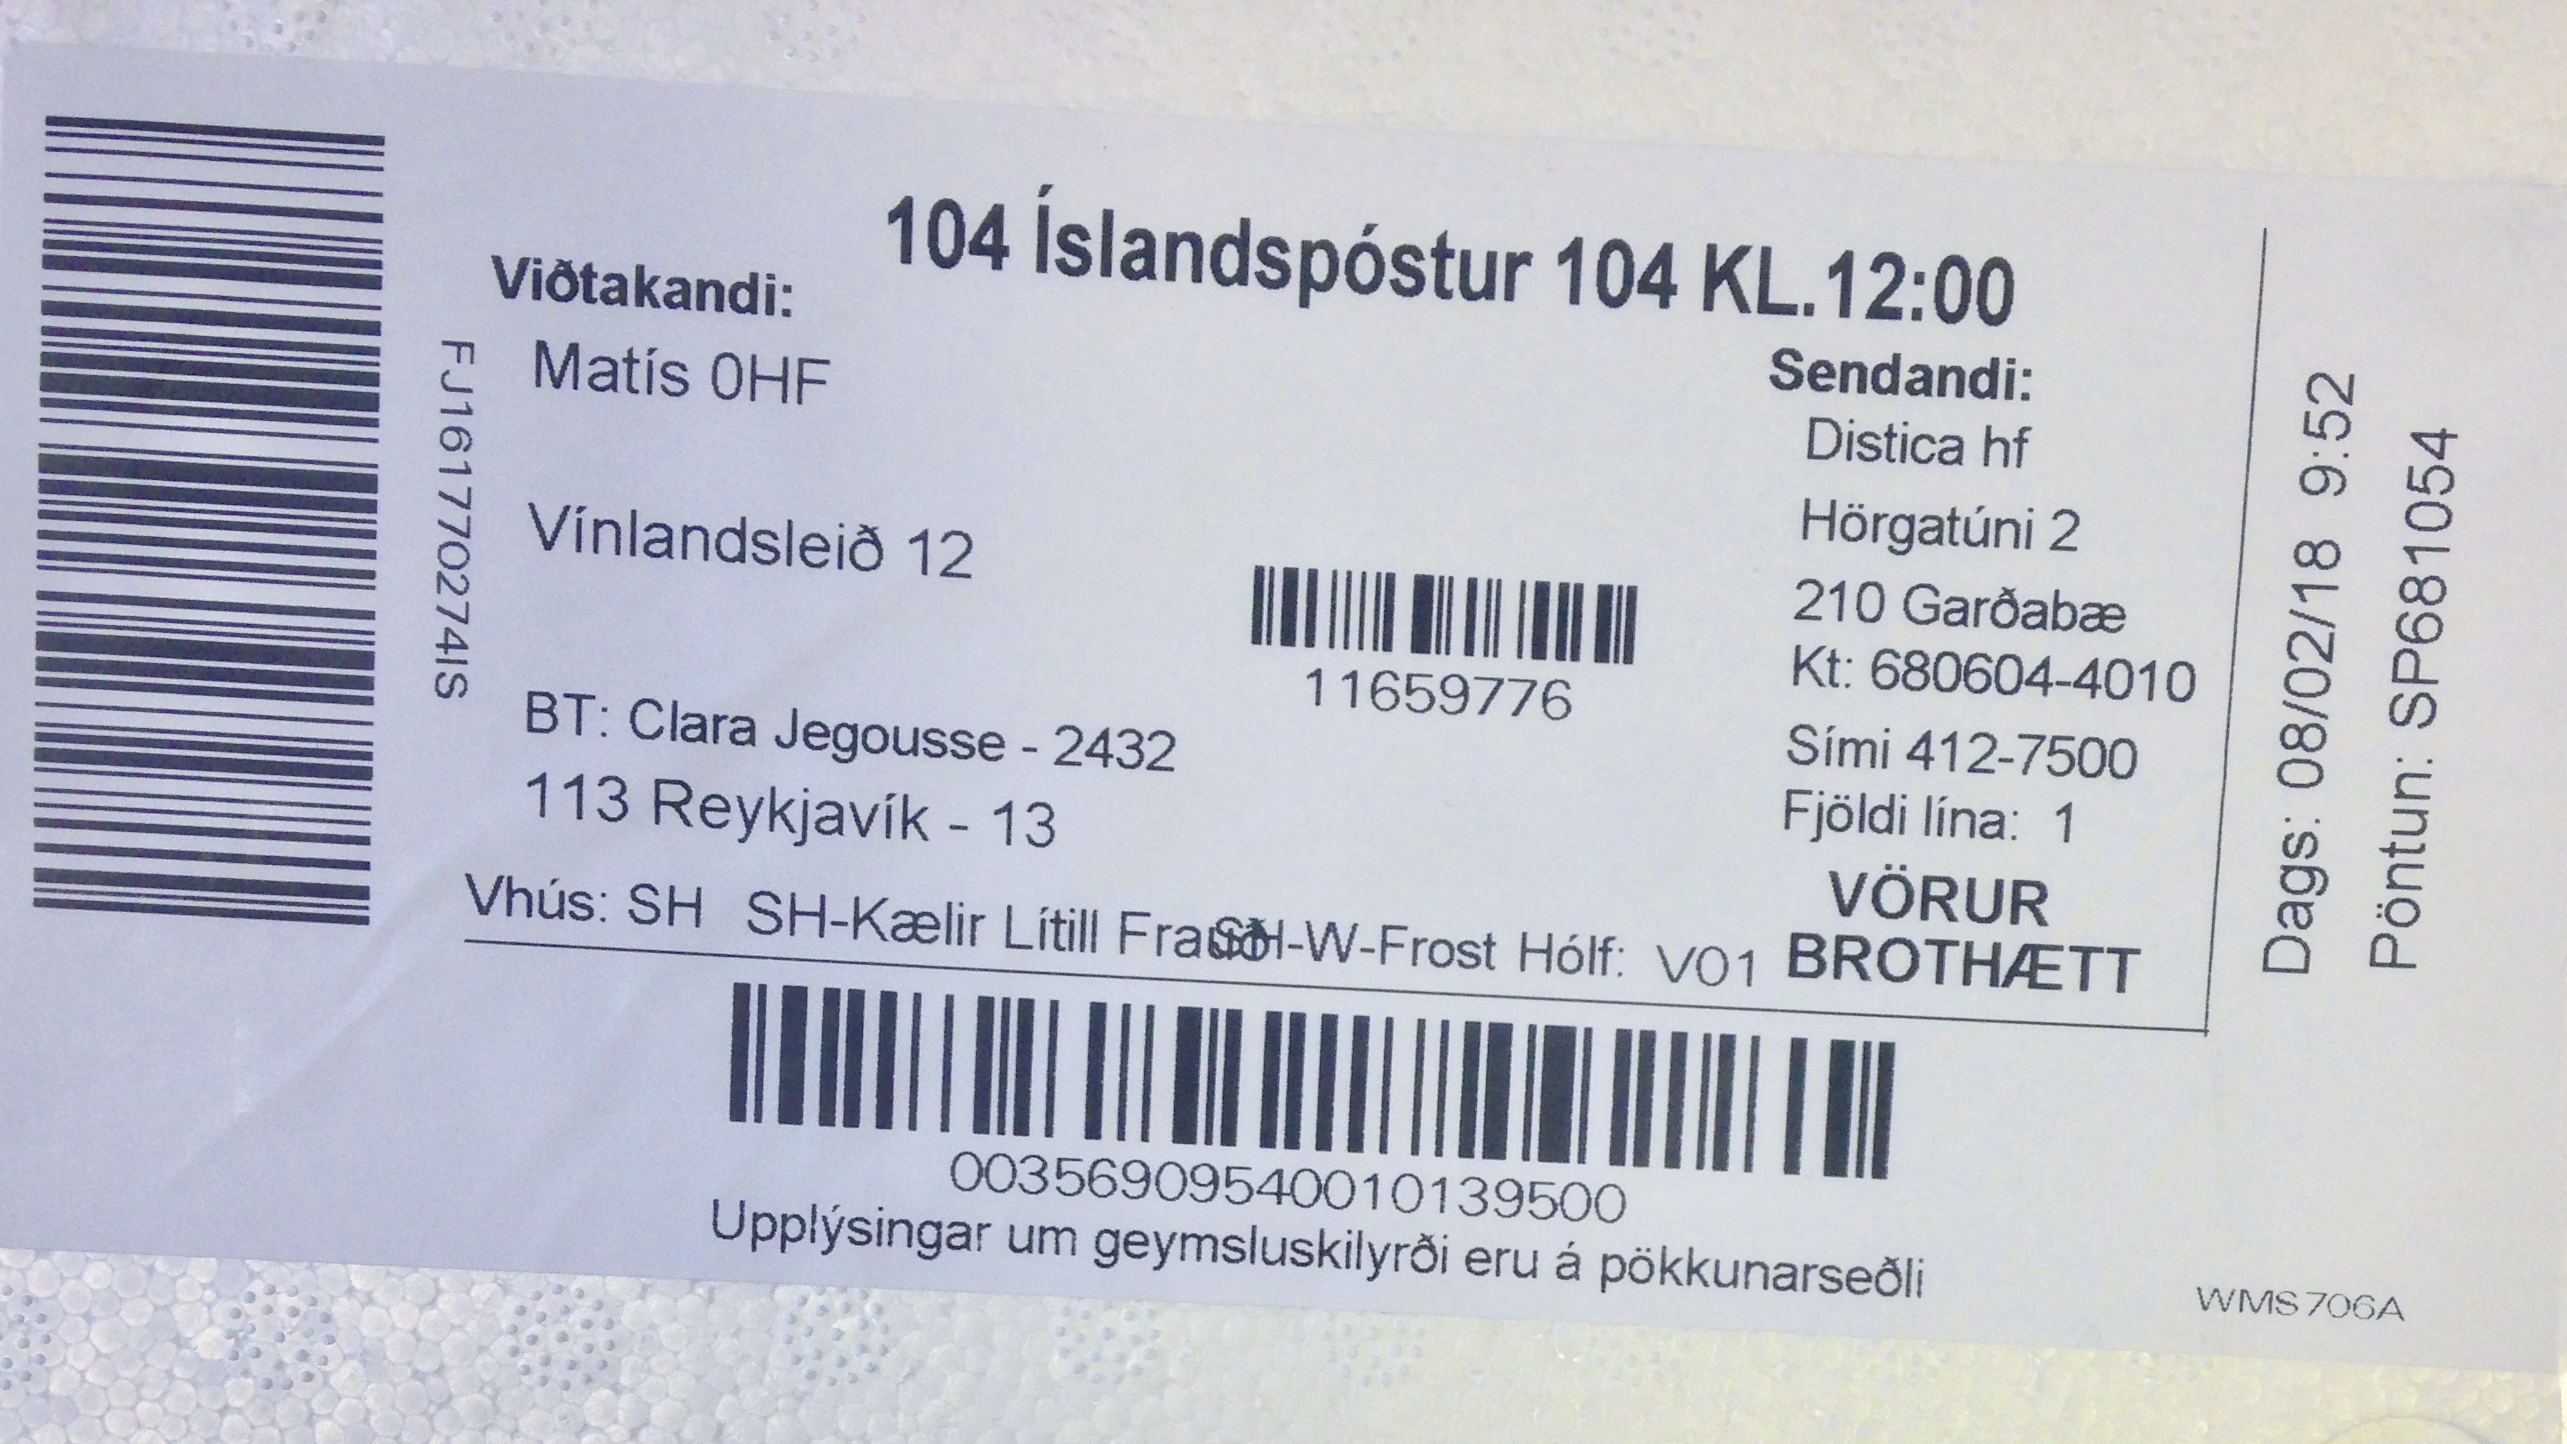
\includegraphics[width=\textwidth]{graphics/pic/20180208_OneTaq_delivery.png}
\end{figure}

\comment{Also we recieved the glutaraldehyde for the winter survey so I also emailed all the persons that helped us getting it on time to thank them for their help.}